%!TEX root = thesis.tex

\section{Motivation}
\subsection{Energy Crisis, Resources and Climate Change}
The energy crisis is one of the most essential and critical crises in the 21st century. Due to the growth of population and the increase of energy intensity per capita, a shortage of energy supply has occurred frequently in recent years, which often causes an energy crisis, usually involving scarcity of oil, electricity or other natural resources. 

Nowadays, non-renewable resource still consists of a large proportion in the energy system. However, according to the BP Statistical Review of World Energy \& Ember (see Figure~\ref{intro_renewable}), the share of electricity production from renewables has continued growing since 2007. In 2020, the share of electricity production from renewables was around 29\% (see Figure~\ref{intro_renewable}). In other words, non-renewables are still the majority sources of electricity production today, although their share is shrinking.

\begin{figure}[!t]
\center
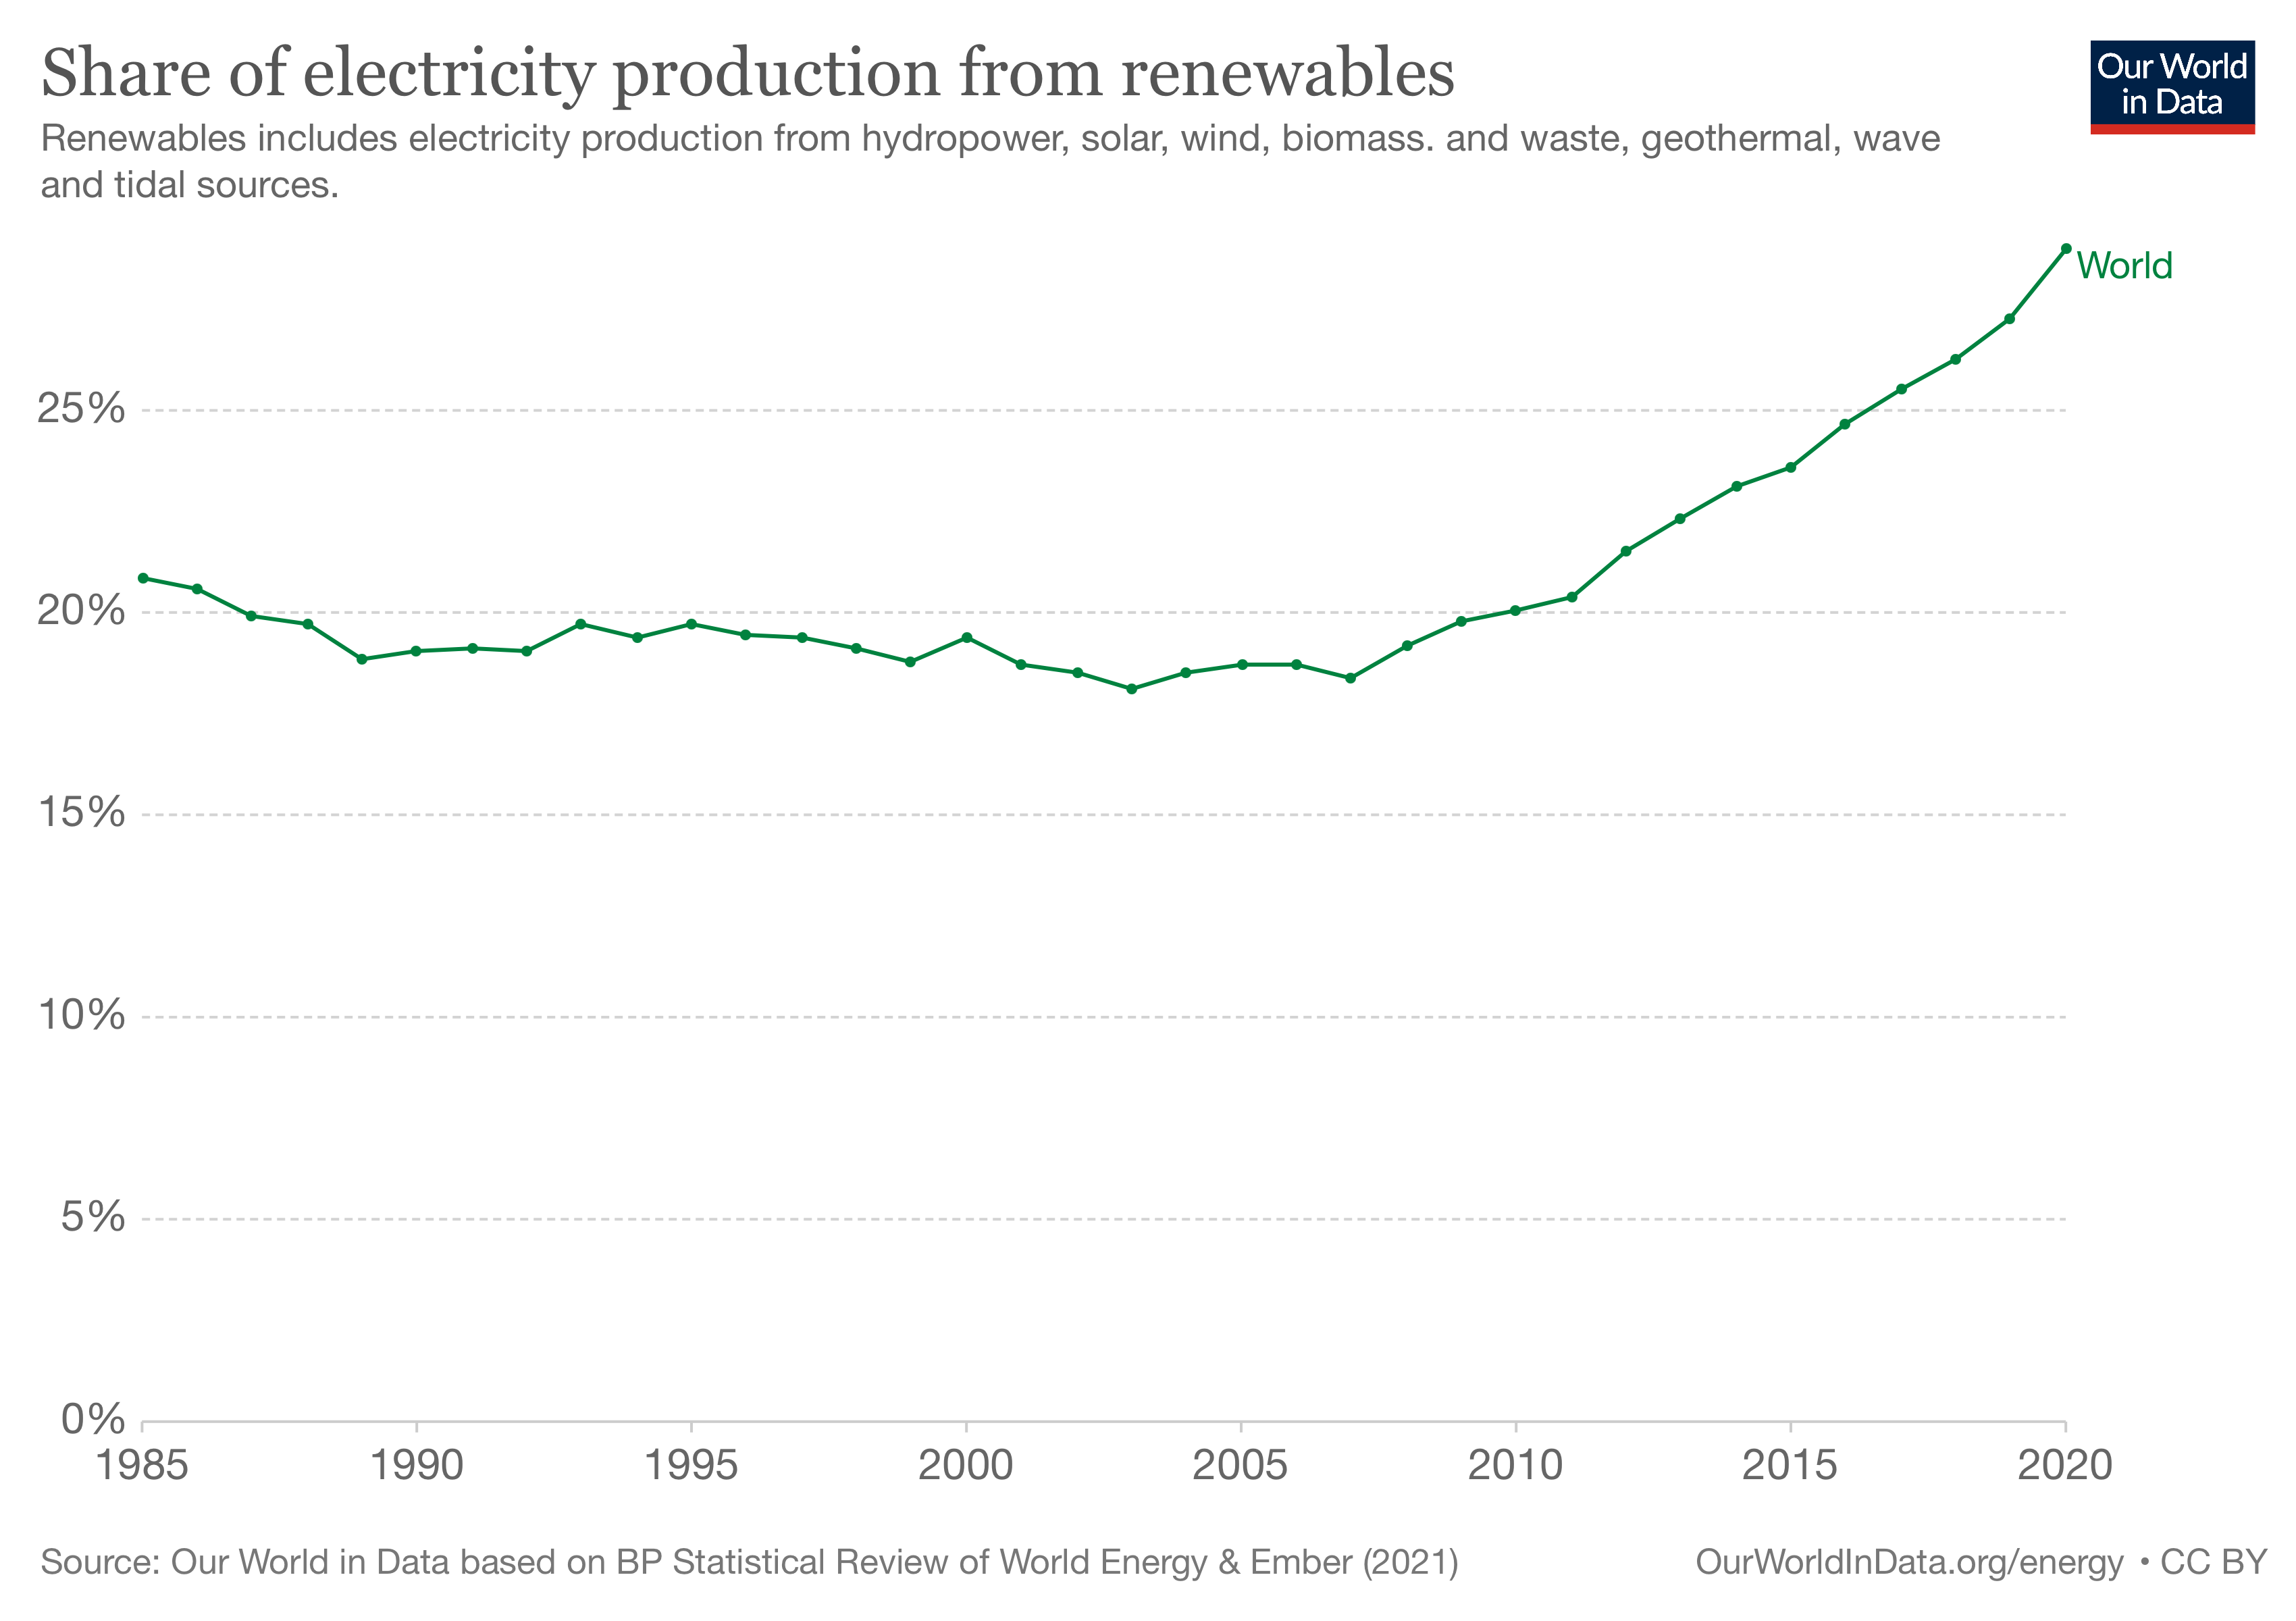
\includegraphics[scale=0.12]{img/intro_renewable.png}
\longcaption{Share of electricity production from renewables.}{The share of electricity production from renewables increased from around 18\% to 21\% during 1985 to 2007~\cite{BP2021bp}. The share of electricity production from renewables has been continually growing since 2007. In 2020, the share of electricity production from renewables was around 29\%.}
\label{intro_renewable} % Figure 1.1
\end{figure}

Although we might not meet the complete depletion of non-renewable resources in the future 50 years, based on Hotelling’s "Economics of Exhaustible Resources", David Ricardo proposed that as the historical production stock accumulates, higher grade ores get depleted, and the producer resorts to lower grade ores, sustaining greater extraction costs~\cite{devarajan1981hotelling}. It means the extraction costs rise, and the price of the products based on ores will rise as well. 


Thus, we can assume that the price of most non-renewable resources, like oil, coal and gas, will rise since these have similar properties with ores. In fact, according to BP Statistical Review 2016~\cite{BP2016bp}, from 1987 to 2015 (from 1989 to 2015 for natural gas), the price of oil, coal and natural gas rose by approximately 36\%, 81\%, and 53\% overall (Figure~\ref{intro_fossil-fuel-price-index}). It is worth mentioning that the final price of any fuel is a complex portfolio of extraction costs, offers and demand affected by different geopolitical events.


\begin{figure}[!t]
\center
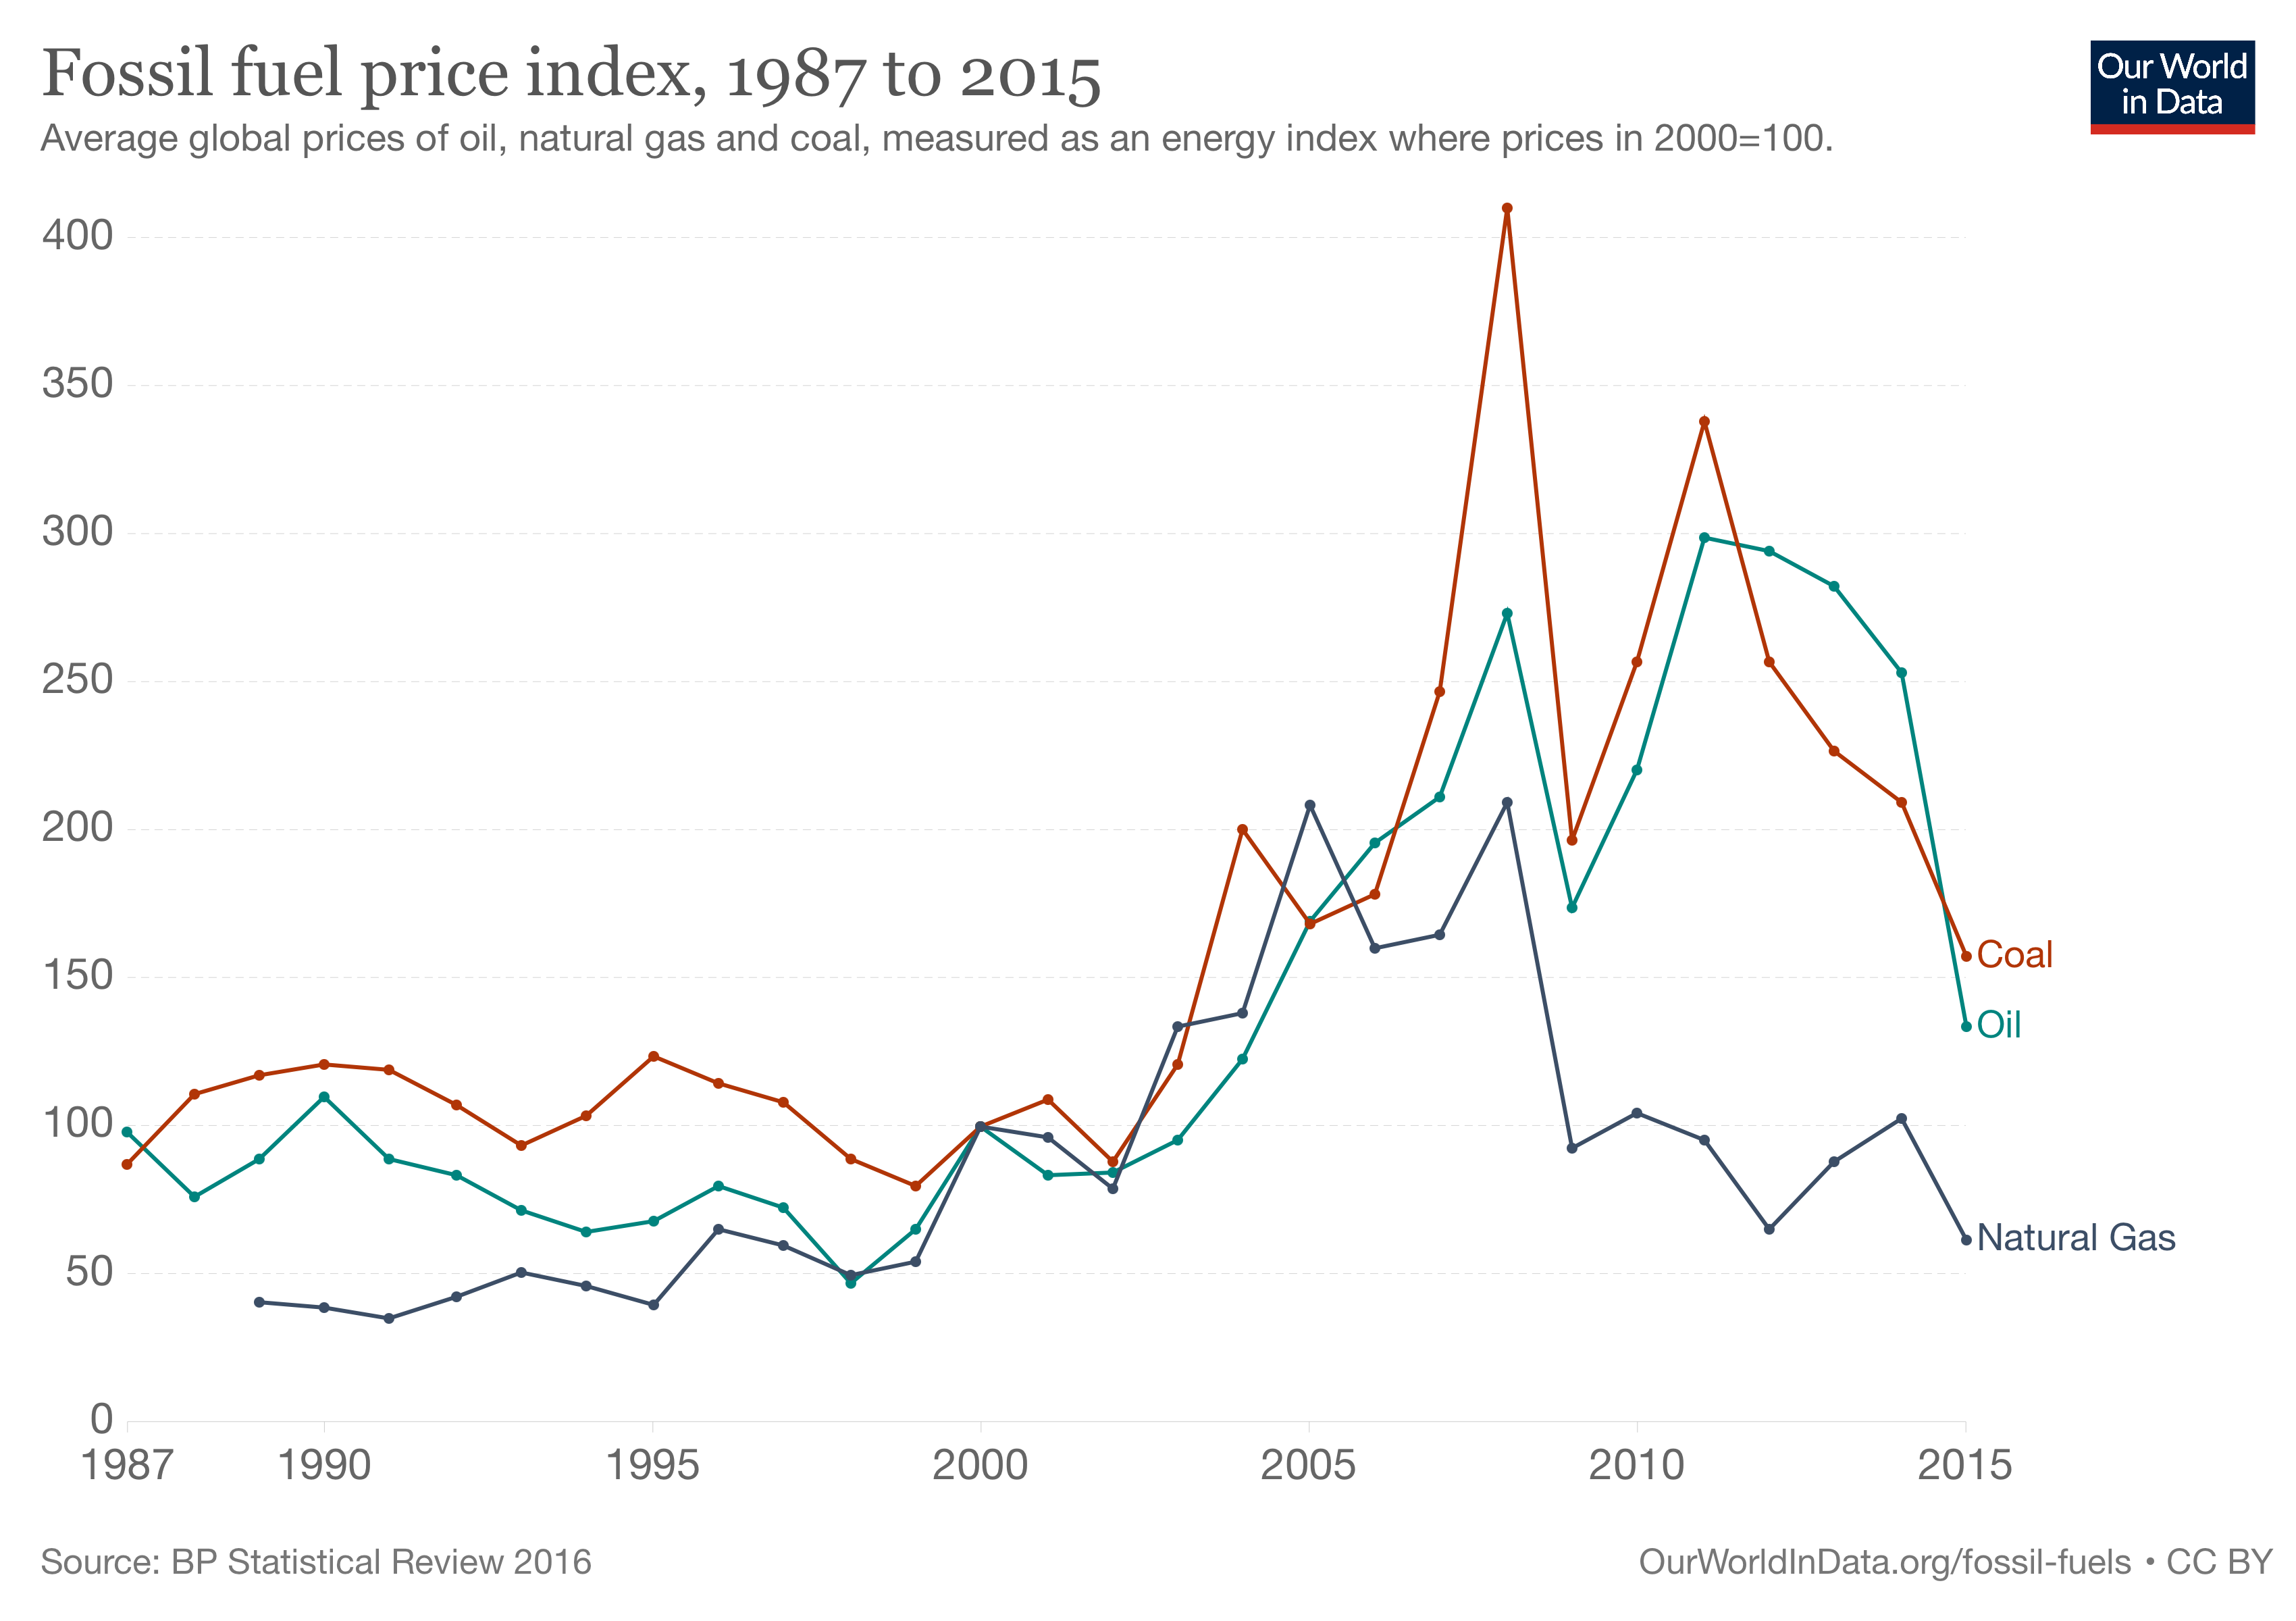
\includegraphics[scale=0.12]{img/intro_fossil-fuel-price-index.png}
\longcaption{Fossil fuel price index, 1987 to 2015.}{Prices of different fossil fuels rose from 1987 to 2015 overall~\cite{BP2016bp}.}
\label{intro_fossil-fuel-price-index} % Figure 1.2
\end{figure} 


In the past 650,000 years, there were seven-cycle glaciers to advance and retreat. However, the climate in the past 70 years has been changed differently from other periods~\cite{parmesan2003globally}. It has already had effects on the environment around us. Glaciers are shrinking, and ice is breaking up earlier on the lakes and rivers. Most climate scientists agree that it is human activities that cause global warming~\cite{epic337530}. The climate on the earth is changing throughout history.\\

As we know, atmospheric \ce{CO2} is a significant component of the atmosphere. However, atmospheric \ce{CO2} had never been above 300 parts per million until 1950 (Figure~\ref{intro_nasa_co2}). 

The atmospheric concentration of \ce{CO2} has been risen for around 36\% from 1914 to 2018 (Figure~\ref{intro_co2-concentration-long-term}).
More than a third has increased atmospheric \ce{CO2} concentration since the Industrial Revolution began~\cite{epic337530}. More importantly, atmospheric \ce{CO2} has exceeded the highest level in the past 400,000 years (Figure~\ref{intro_nasa_co2}), and it was 408.52 ppm in 2018 (Figure~\ref{intro_co2-concentration-long-term}).


\begin{figure}
\center
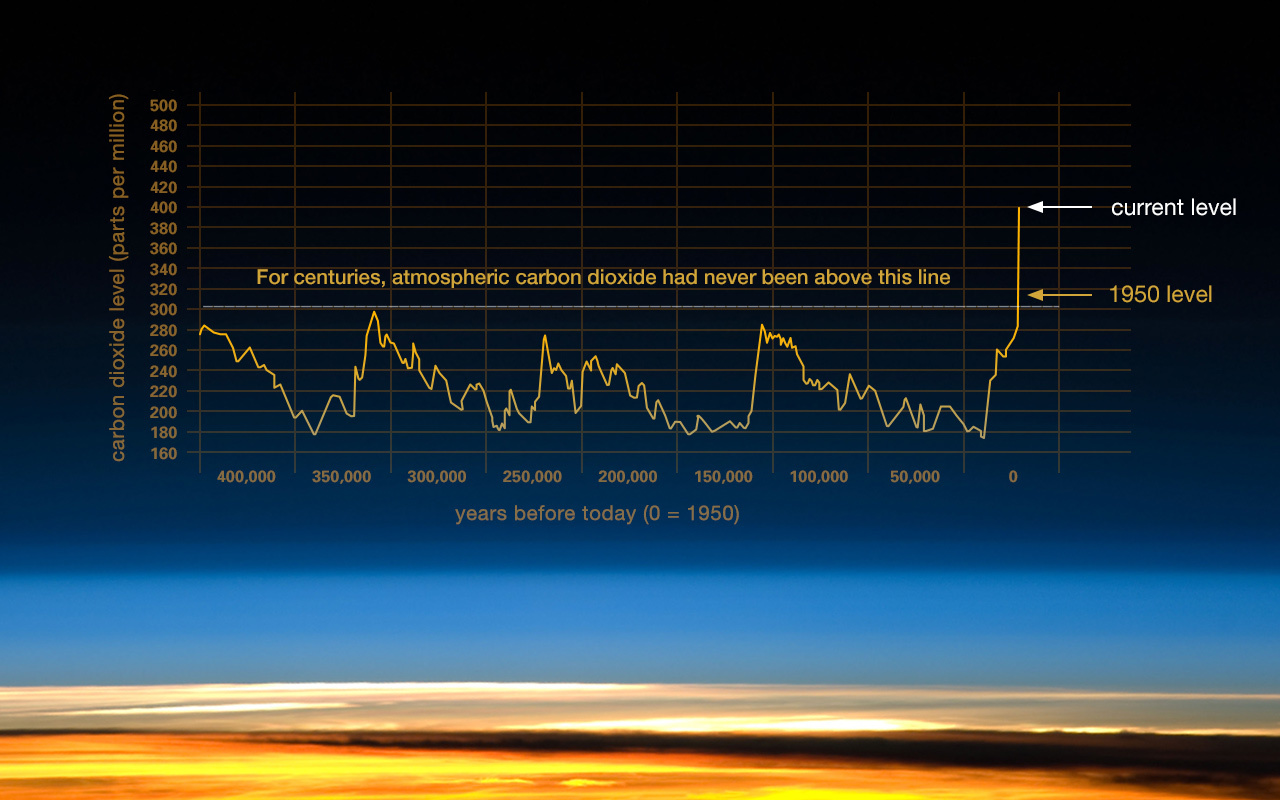
\includegraphics[scale=0.28]{img/intro_nasa_co2.jpeg}
\longcaption{The evidence that atmospheric \ce{CO2} has increased since the Industrial Revolution began}{\label{intro_nasa_co2} The evidence that atmospheric \ce{CO2} has increased since the Industrial Revolution began. Image courtesy: https://climate.nasa.gov/evidence} % 1950

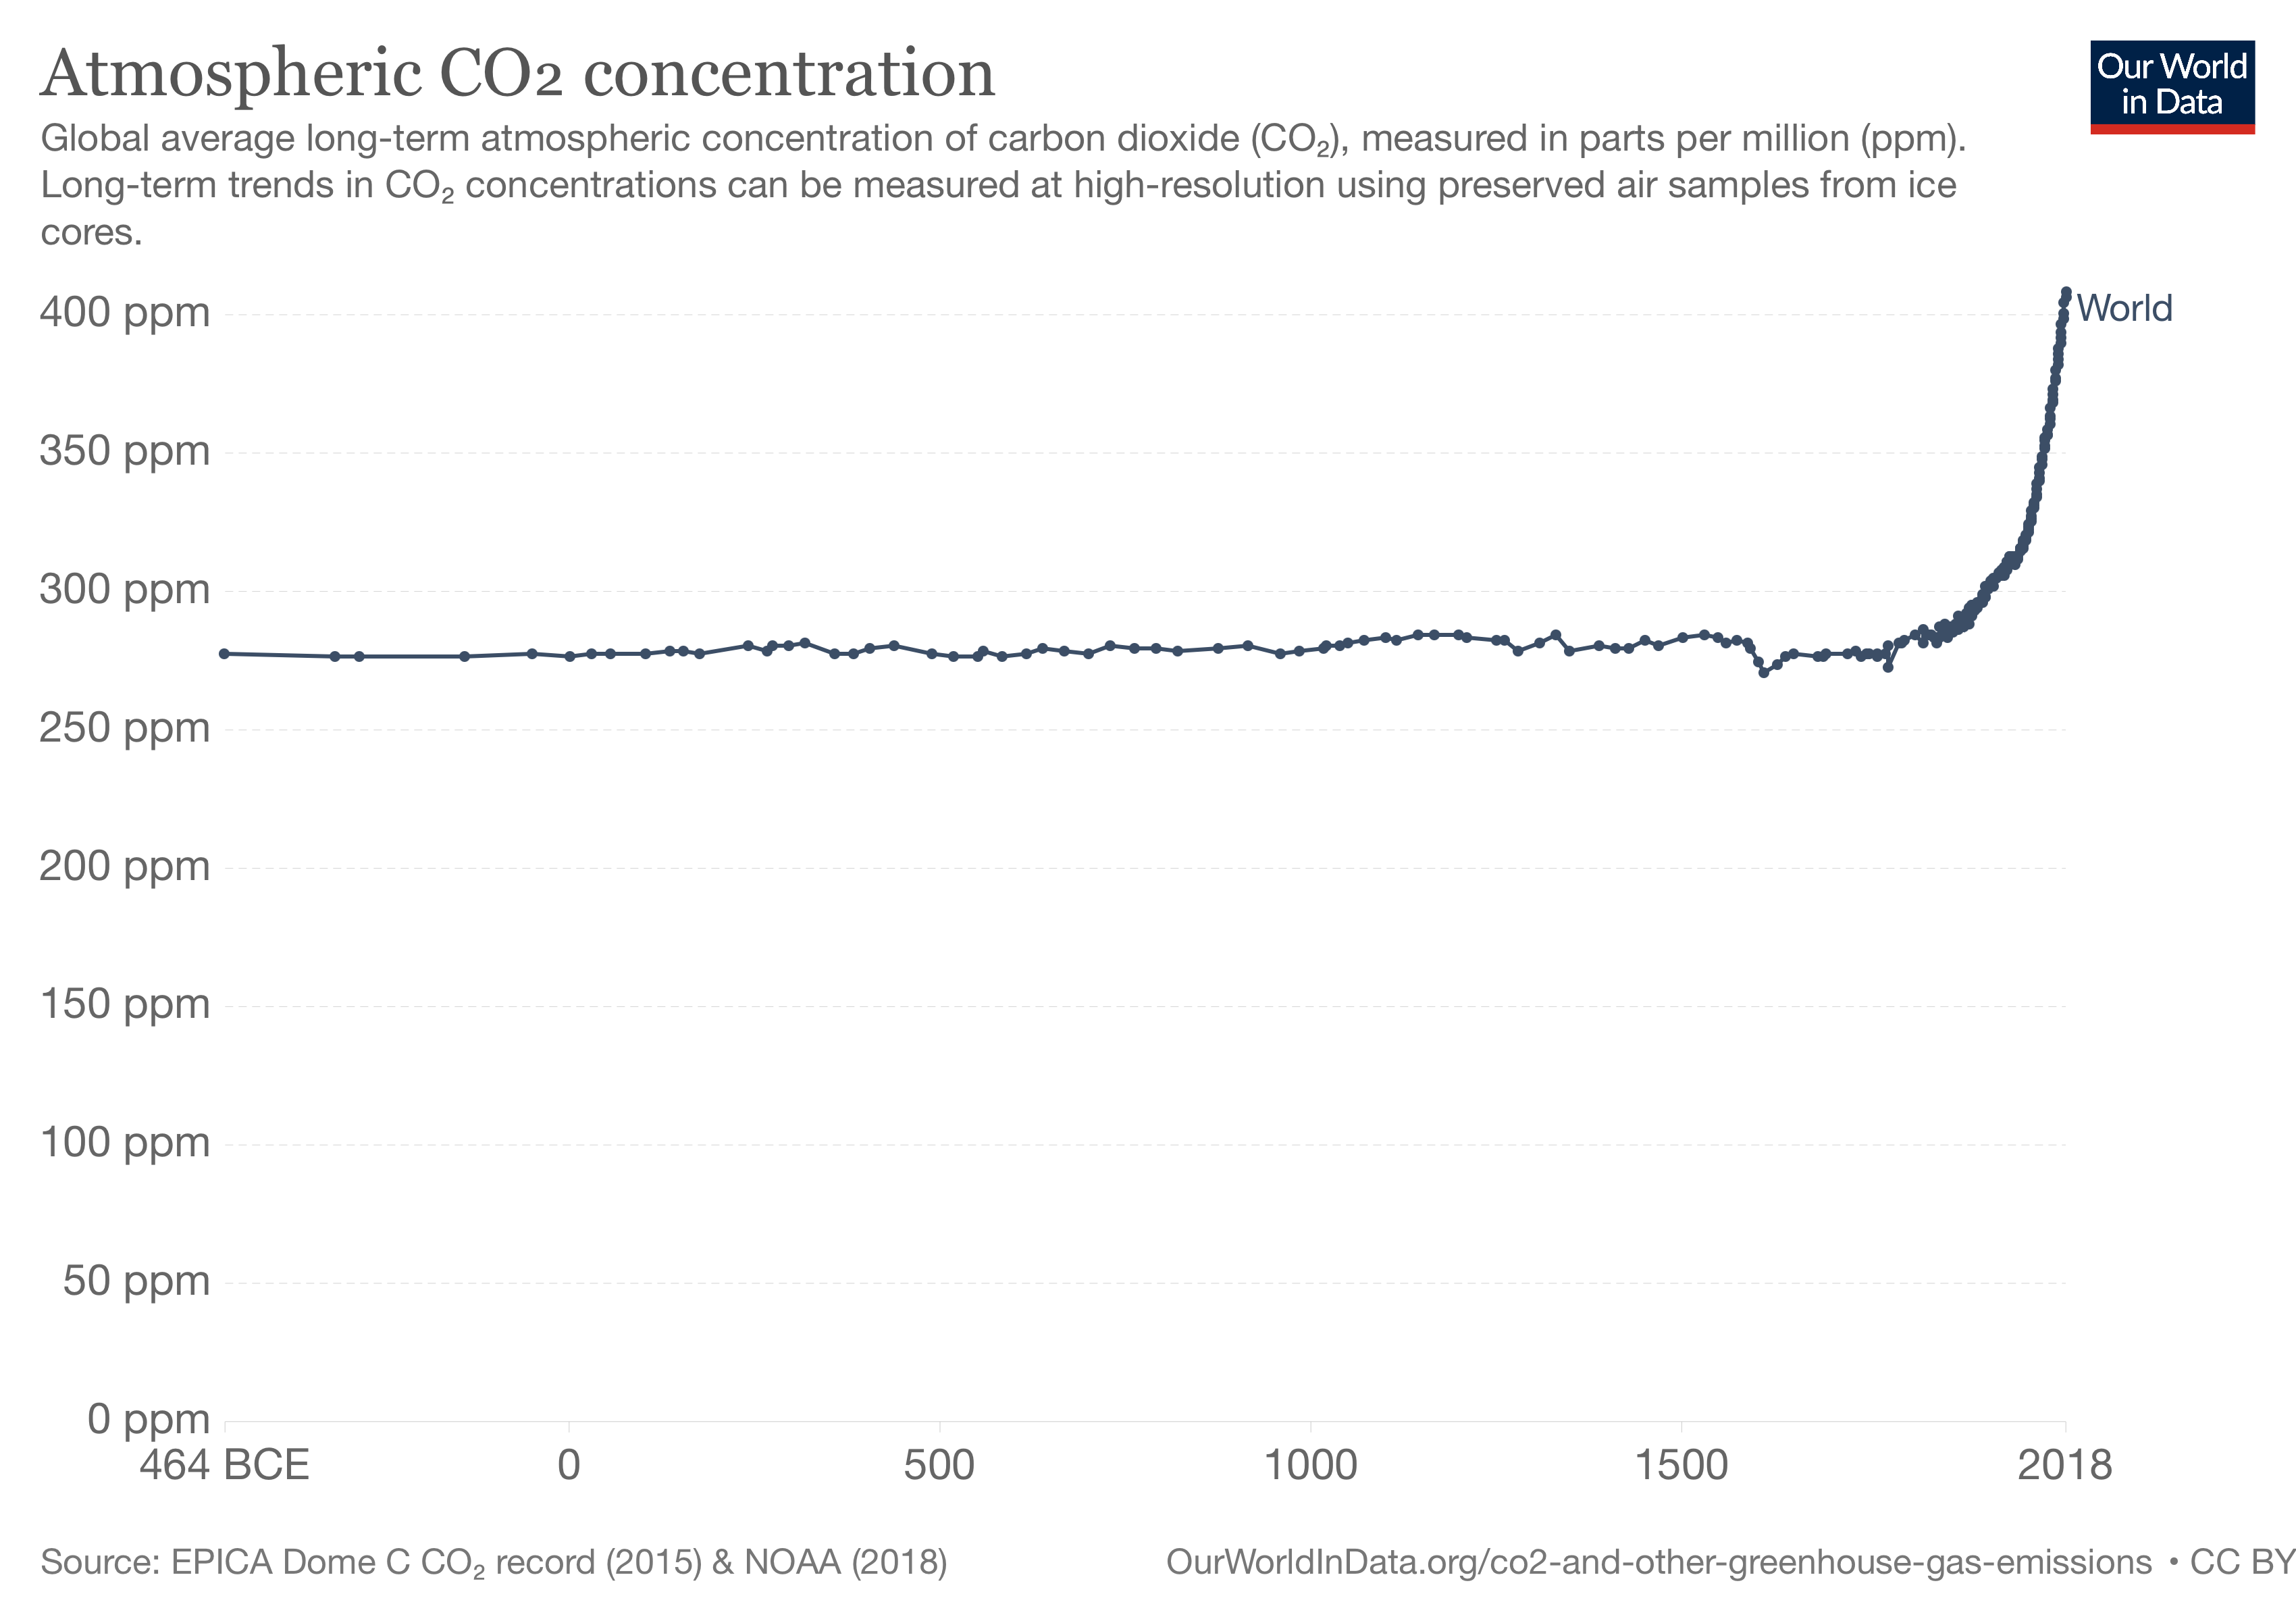
\includegraphics[scale=0.12]{img/intro_co2-concentration-long-term.png}
\longcaption{Atmospheric \ce{CO2} concentration.}{Atmospheric \ce{CO2} concentration in 1914: 300.17ppm; Atmospheric \ce{CO2} concentration in 2018: 408.52ppm.}
\label{intro_co2-concentration-long-term}
\end{figure}




% Page 5
\newpage
In summary, the rising energy demand and lack of energy supply may cause a short-term energy crisis. The finite resources of fossil energy will drive the price of electricity and consumer goods to rise. Moreover, the burning of fossil energy will cause excessive emissions of greenhouse gases, leading to global warming. However, a door opens for cheaper but unpredictable renewable energy due to more expensive fossil fuels. According to Paris Agreements~\cite{unies2015accord}, it is vital to reduce the emissions of fossil energy on a large scale in every sector of human activities. To respond to climate change, supporting the United Nations Sustainable Development Goals and taking urgent action to address climate change and its impact, the International Maritime Organization has formulated a timetable to reduce greenhouse gas emissions from international shipping.~\cite{joung2020imo} It pointed out that between 2030 and 2050, the carbon intensity of the fleet will be reduced by at least 70\%~\cite{joung2020imo}. Before 2050, the total annual greenhouse gas emissions will be reduced by at least 50\%, which requires a reduction of approximately 85\% of carbon dioxide per ship~\cite{joung2020imo}. 

\subsection{Small-Boat Fleet and Emission Inventory}
Emission inventories for small vessels, including small fishing vessels are not developed for all years hence it is necessary to make the assumption of the emission growth for this class. In 2018, total shipping \ce{CO2} emissions increased to 1056 million tonnes compared to 962 million tonnes in 2012~\cite{IMO2021Fourth}.
In 2016, total \ce{CO2} emissions of the industrial fishing sector were 159 million tonnes, and the small-scale fishing sector emitted 48 million tonnes~\cite{GREER2019103382}. Suppose the increase rate of \ce{CO2} in 2018 was the same as the rate in 2016, and the ratio of the number of small boats and the number of boats can be approximate as the ratio of the number of small fishing boats and the number of fishing boats. Then in 2018, the total \ce{CO2} emissions for the small boat fleet can be calculated as 318.8 million tonnes.

Small vessels are classified as those smaller than 24 meters~\cite{uk2021Operational}. Knowing the shipping sector's emissions inventory can help understand what measures need to be taken to enable the industry to start the road to full decarbonization. Although it is possible to calculate large vessels from the international registry system and use the satellite data sent from the ship's transponder to account for the large vessels~\cite{IMO2021Fourth}, the small vessels depend on the national registration system, and their operation is assumed. In addition, there are many types of small vessels fleets such as machinery (e.g. fishery, people carrier, etc.), hull shape and structure, and the activities of owners and operators. The diverse small boat fleet operational profile is increasing the challenge of accurately accounting for their emission inventories.

Emissions from the global fishing industry grew by 28\% between 1990 and 2011, with a minor coinciding increase in production; however, marine fisheries are typically excluded from international assessments of \ce{CO2} or are generalized based on a limited number of case studies~\cite{parker2018fuel}. Developed economies such as the UK have a national registry~\cite{uk2021registration} that allows to have a sense of the level of small boat activity and hence infer the \ce{CO2} emissions.

However, in developing countries, it tends to be a mixed bag on the level of precision and availability. For instance, in Mexico, only fishing vessels are counted into registry~\cite{Mexico2021RegisteredVessels}. Still, it is difficult to know where they are located. Besides, the rest of the small-boat fleets are not considered. In all, Mexico does not have a regional \ce{CO2} inventory considering the small-boat fleet. Therefore, quantifying the number of small-boat fleets will allow a better precision of where the emissions are being emitted and will be the focus of understanding the emission inventory of the shipping sector.


Observing the shipping activity in the Gulf of California is essential due to its unique geographical location, conformation, and biophysical environment ~\cite{LLUCHCOTA20071, munguia2018ecological, MARINONE2012133}. In the Gulf of California, there is the largest fish producing state (Sonora) in Mexico~\cite{MELTZER2006222} and the most prominent sports fishing destination (Los Cabos, Baja) in Mexico~\cite{hernandez2012economic}. Besides, the Gulf of California has a faster shipping route to mainland Mexico than from Yucatán Peninsula.

\subsection{Bringing Convolutional Neural Networks in Satellite Images Detection}
Bringing convolutional neural networks to the field of satellite image recognition is important. First, the threshold of satellite image recognition is gradually decreasing. As the quality and quantity of global satellite images improve, obtaining the same or even better detection results with reduced parameters and complexity of convolutional neural networks is possible. Second, satellite image recognition is not new. A current PhD at the University of Texas at Austin focuses on using machine learning and remote sensing imagery to discover undersea shipwrecks ~\cite{character2021archaeologic}. However, as Figure~\ref {fig:shipwrecks} shows, discovering submarine wrecks does not require algorithms to describe the location and size of the wreck very precisely, as opposed to precisely identifying and measuring the length of a small boat. Therefore, in this thesis, accurately measuring the dimensions of small ships is definitely a challenge and a rewarding thing to do.

\begin{figure}[!t]
    \centering
    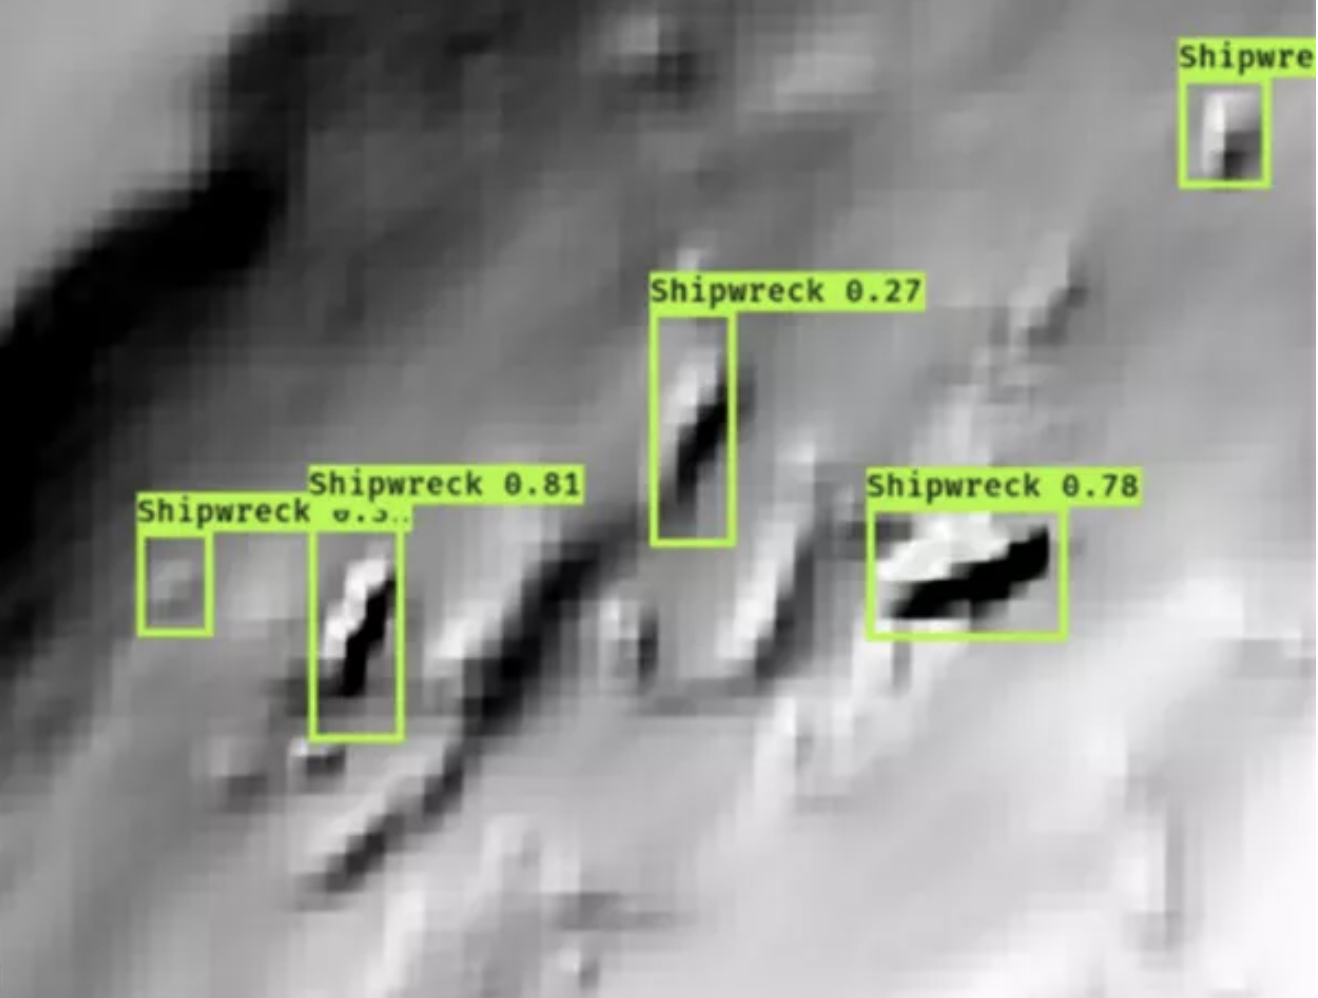
\includegraphics[scale=0.5]{img/shipwrecks.png}
    \caption{The hillshade image of the sonar or lidar output by the model.}
    \label{fig:shipwrecks}
\end{figure}


\newpage
\section{Research Questions}
This article aims to determine whether image recognition such as convolutional neural networks can be used to successfully find boats with a length of 24 meters or less on the sea surface, and classify the boats according to their attributes.

Although the object detection technology based on convolutional neural networks is now mature, it is not easy to measure accurately to the centimeter level. Should convolutional neural network or image recognition technology be an effective solution? If effective, can this method be extended to a larger sea area to detect more different types of boats? The research questions to be completed in this paper are detailed as follows:

\begin{enumerate}[(a)]

    \item What is the small-boat fleet numbers and composition around the Gulf of California?
    
    \item How accurate is the image machine-learning algorithm that recognises the small boat?
    
    \item How this algorithm can be scaled up for the rest of Mexico/west coast of the U.S.A.?
\end{enumerate}



\newpage
\section{Thesis Outline}
Following the three research questions that we just discussed, this thesis consists of four parts --- \sys{Chapter 2 Literature Review}, \sys{Chapter 3 Methodology}, \sys{Chapter 4 Results}, and \sys{Chapter 5 Conclusions and Future Work}.

\begin{description}
    \item In Chapter~\ref{chap:2}, I will begin with an overview of recent developments in identifying small boats and shipping decarbonisation. Next, I will briefly discuss developing convolutional neural networks and algorithms for cloud removal for satellite images.

    \item In Chapter~\ref{chap:3}, I will talk about the algorithms I used in this project and their mathematical foundations, such as convolutional neural networks. Then, I will discuss the data sources. For example, how to improve the original data specification to fit an existing deep learning framework. Likewise, I will briefly introduce the advantages of GPUs. This will enable the reader to understand the mathematics behind this decision to use GPUs. Then, I will talk about everything about detection and classification. First, I will start by defining the scope of recognition. I will explain why I selected only some of the cities in the Gulf of California. Then, I will discuss the quality of the data provided by Google Earth Pro and the principles and effects of sharpening images using image kernels. Finally, I will explain the principle of detecting the length of small boats and the thinking behind classifying small boats. At the end of this chapter, I will include a workflow on the algorithm.
    
    \item In Chapter~\ref{chap:4}, I will discuss the logs and the length of the detected boats when training the convolutional neural network. Importantly, I will also analyze the composition of the small boats in the three port cities and the potential reasons for this.
    
    \item In Chapter~\ref{chap:5} and Chapter~\ref{chap:6}, I will discuss a few pressing issues to be addressed in the future and summarize the conclusions reached and the progress made.
\end{description}


\newpage
\section{Contributions}
The contributions of this thesis are summarized as follows:
\begin{itemize}
    \item The accuracy of my trained object detection algorithm can reach 96\% to 98\%.

    \item I proposed and implemented an algorithm for measuring the length of an object (small boat) based on object detection, which showed excellent accuracy in tests.

    \item I proposed and implemented the algorithm to determine whether the detected small boat is a domestic recreational small boat, dividing small boats into domestic recreational small boats and fishing boats. Although the algorithm has flaws, this is an attempt to use a pure computer vision algorithm rather than a neural network in identifying objects. Nevertheless, I believe this is the first but important step in constructing a way to identify the types of small boats. Based on this, I answered questions about the composition of small boats in the Gulf of California.

    \item I developed Python scripts that can count the number of small boats, the number of large boats, and the number of small boats for home recreation. This automated the statistics and saved a great deal of time in counting.

\end{itemize}